\documentclass{article}
%     \PassOptionsToPackage{numbers, compress}{natbib}
% before loading neurips_2019

% ready for submission
%\usepackage{neurips_2019}

% to compile a preprint version, e.g., for submission to arXiv, add add the
% [preprint] option:
\usepackage[preprint]{neurips_2019}

% to compile a camera-ready version, add the [final] option, e.g.:
%     \usepackage[final]{neurips_2019}

% to avoid loading the natbib package, add option nonatbib: hjjhhhjhjhj
%     \usepackage[nonatbib]{neurips_2019}

\usepackage[utf8]{inputenc} % allow utf-8 input
\usepackage[T1]{fontenc}    % use 8-bit T1 fonts
\usepackage{hyperref}       % hyperlinks
\usepackage{url}            % simple URL typesetting
\usepackage{booktabs}       % professional-quality tables
\usepackage{amsfonts}       % blackboard math symbols
\usepackage{nicefrac}       % compact symbols for 1/2, etc.
\usepackage{microtype}      % microtypography
\usepackage{comment}
\usepackage{wrapfig}
\usepackage[normalem]{ulem}
\usepackage{times,amssymb,amsmath,amsfonts,openbib,multirow}
\usepackage{comment}
\usepackage{times}
\usepackage{graphicx}
%\usepackage{subfigure}
\usepackage{subfig}
\usepackage{setspace}
\usepackage{afterpage}
\usepackage{url}
\usepackage{caption}
%\usepackage{subcaption}
%\usepackage{listings}
%\usepackage{amsthm}
%\usepackage{cite}
\usepackage{amsmath}
%\usepackage{algorithm}
%\usepackage{algorithmicx}
%\usepackage[noend]{algpseudocode}
\usepackage{xcolor}
\usepackage[linesnumbered,ruled,vlined]{algorithm2e}

\usepackage{authblk}
\usepackage[english]{babel}
\usepackage{blindtext}

\newcommand{\todo}[1]{{\color{red}\bf[[#1]]}}
\newcommand{\scheme}{SPAL}

\title{ \scheme: {\underline S}tock {\underline P}rices Forecast with  Stacked {\underline A}utoencoders and {\underline LSTM} 
}
%{\underline E}volutionary {\underline S}ynthesis of {\underline P}rograms}



\author[]{Shantanu Mandal \thanks{shanto@tamu.edu}}
\author[]{Jee Su Byun \thanks{jb733@tamu.edu}}
\author[]{Zebo Xiong \thanks{dior@tamu.edu}}
\affil[]{Texas A\&M University}
\renewcommand\Authands{ and }

\begin{document}

\maketitle
\begin
{abstract}
The application of neural network (NN) methods in finance has received a great deal of attention from both industry and academia ~\cite{bao2017deep}. This study presents an integrated analysis which combines stacked autoencoders, long short term memory (LSTM) and feature analysis with embedded NN. LSTM networks are originally designed for sequential learning but are less commonly used in financial time series predictions; yet, they are inherently suitable for this domain~\cite{fischer2018deep}. We deployed LSTM networks for predicting out-of-sample directional movements for the constituent stocks of the S\&P500 from 2009 until 2018. According to the result, outperformance relative to the general market is very clear from 1992 to 2009, but as of 2010, excess returns seem to have been arbitraged away with LSTM profitability fluctuating around zero after transaction costs. We further unveil sources of profitability, thereby shedding light into the black box of artificial neural networks. The neural network has three stages. {\em First}, the stock price time series is decomposed by WT to eliminate noise. {\em Second}, SAEs is applied to generate deep high-level features for predicting the stock price. {\em Third}, high-level denoised features are then fed into LSTM to forecast the next day's closing price. S\&P500 index and their corresponding index futures are chosen to examine the performance of the proposed model. 
%Finally we compared the performance with other techniques such as SVM, SVR and XGBoost. 
\end
{abstract}

\section{Introduction}
\label{sec-intro}
Stock market prediction is usually considered as one of the most challenging issues among
time series predictions~\cite{wang2012novel} because of its volatile properties. How to correctly predict stock movement is still an heated topic with respect to the economic and social organization. During the past decades, machine learning techniques, such as Artificial Neural Networks ~\cite{chen2014deep} and the Support Vector Regression (SVR) ~\cite{guo2014feature}, have been widely used. In the paper, however, we try to do experiments on an improved model which models complex real-world
data by extracting robust features that capture the relevant information ~\cite{bao2017deep}. Considering the complexity of financial time series, neural network is regarded as one of the most charming topic ~\cite{bao2017deep}. However, this field still has much to explore.  

Currently we have three main neural network approaches. First, convolutional neural networks. Second,  deep belief networks. Third, stacked autoencoders. Previously, the relevant methods used for finance were the former two of these. For example, Ding et al. ~\cite{ding2015deep} combine the neural tensor network
and the deep convolutional neural network to predict the short-term and long-term influences
of events on stock price movements. Also, certain works use deep belief networks. 

However, there has been only one attempt, by Bao et al. ~\cite{bao2017deep}, that incorporates stacked autoencoders. This paper will continue to explore Bao's paper to refine the stock prediction. Bao's model has three parts: wavelet, stacked autoencoders(SAEs) and LSTM. SAEs play a main role in that model. It is used to learn the deep features of a stock price in an unsupervised way, as SAEs model can successfully learn invariant and abstract features ~\cite{chen2014deep}.

After SAE is used to find the invariants, LSTM is then used to enhance the prediction accuracy. It is one of the most advanced deep learning architectures for sequential learning tasks, such as handwriting recognition, speech recognition, or time series prediction ~\cite{fischer2018deep}. Surprisingly, its application in financial area has yet been little and there has not been any previous attempt to deploy LSTM networks on a large, liquid, and survivor-bias-free stock universe to assess its performance in large-scale financial market prediction tasks ~\cite{fischer2018deep}. Unlike conventional RNN, LSTM is well-suited to learn from experience to predict time series when there are time steps with arbitrary size. In addition, it can solve the problem of a vanishing gradient by having the memory unit retain the time related information for an arbitrary amount of time ~\cite{how2016behavior}. Previous work has shown that LSTM is more effective than RNN. At the same time, WT is used to fix the noise feature of financial time series. We use it to denoise the input financial time series. We'll call this model \scheme\ hereafter ~\cite{bao2017deep}.

We select S\&P500 Index for our experiments from the past 10 years, up until 2018 and use \scheme\ to forecast the movements of each stock index and check how well our model is performing in predicting stock moving trends. In the future, we hope to test the performance of the model in multiple financial markets instead of only one market for better results. This is because, according to the efficient market hypothesis (EMH), the efficiency of a market affects the predictability of its assets. In other words, even though we may achieve satisfactory predictive performances in one market, it is still difficult to attribute it to the role of the proposed model~\cite{bao2017deep} in other financial markets. Since we will eventually test the model in multiple market conditions, we hope it will help us to solve this problem and proves the robustness of the model. We evaluate the model's performance by measuring how predicted prices are numerically close to the actual prices. There are four possible ways to predict the accuracy: Mean absolute percentage error (MAPE), correlation coefficient (R), Theil's inequality coefficient (Theil U), Root Mean Square Error (RMSE) ~\cite{bao2017deep}. They are widely used to measure the predicted values ~\cite{hsieh2011forecasting}.

 
 
 
 
 
 
 



%In Section ~\ref{sec-problem} we formalize the problem we are solving.  In Section ~\ref{sec-desc} we describe our solution to the problem.  Lessons learned are discussed in Section ~\ref{sec-lessons}.  Results are presented in Section ~\ref{sec-results} and comparisons made to related work in Section ~\ref{sec-rel}.  Finally, we draw conclusions in Section ~\ref{sec-conc}.

%For a given gene, the neural 
%network predicts properties such as how many functions might be common between this gene 
%and the solution or what is

%partly caused by the difficulty in finding appropriate fitness function. To overcome this %difficulty, this paper contributes with a novel approach 
%%to design fitness functions, 
%which is to use a neural network
%as a fitness function. Based on this idea, we propose an evolutionary framework to synthesize %program. The framework, called ESP, contains three novel contributions. 
%Among various machine learning
%bases synthesis techniques, Neural Program Synthesis
%techniques are particularly interesting because such
%techniques can produce actual programs by conditioning a neural network with input-output examples~\cite{}.

%Machine learning based program synthesis can be broadly categorized as Neural Program Induction techniques and Neural Program Synthesis technqiues. Neural Program Induction techniques~\cite{} strive to design a neural network that learns to produce outputs from a latent program representation. On the other hand


\section{Problem Statement}
\label{sec-problem}
%We now formally define the problem statement and the Domain Specific Language (DSL).

%\subsection{Problem Formulation}
%\label{sec-problem}

In this section we will describe 
\begin{itemize}
    \item Basic concepts of the stock bar and pattern and describe why it is hard to get the features.
    \item Why we use NN in detecting stock pattern. 
\end{itemize} 

\begin{figure}[htpb]
\begin{center}
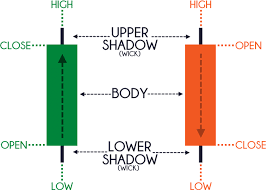
\includegraphics[width=0.4\textwidth]{./figs/candlestick}
\vspace{-0.2cm}
\caption{Stock bar for any timeframe \cite{chartpattern}}
\label{fig_bar}
\end{center}
\vspace{-0.4cm}
\end{figure}

\subsection{Stock series data}
A 'tick' is defined as a single movement in price at any given time frame. As it is very difficult and expensive to collect the tick data history, we used data with larger timeframes in our experiments. A candle bar is commonly used to depict price movement behaviors in a unit timeframe. A bar has 4 data points. Open, high, low, close, as shown in Figure \ref{fig_bar}.

\subsection{Chart pattern}
When seen in multiple timeframes, stock prices follow different chart patterns that indicate certain future price movements with high likelihoods. Before the advent of machine learning in finance, statisticians made predictions by recognizing these patterns. Some of the well known examples of chart patterns are given in figure \ref{fig_pattern}. Since they are not always easily detected with bared eyes, we are motivated to use NN to detect the patterns. As NN is known to capture fuzzy features from large datasets, we can conclude that NN can also predict results with empirical evidence from the past price movements such as these patterns. 


\begin{figure}[htpb]
\begin{center}
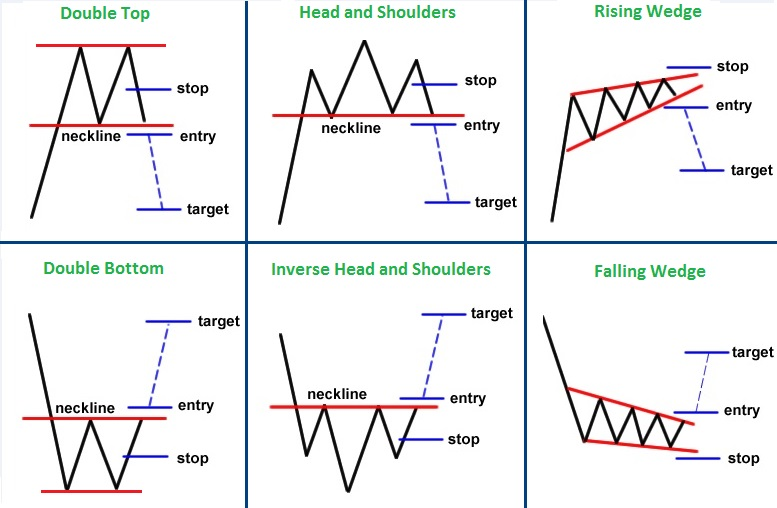
\includegraphics[width=0.9\textwidth]{./figs/chart-patterns}
\vspace{-0.2cm}
\caption{Different stock pattern across timestep \cite{chartpattern}}
\label{fig_pattern}
\end{center}
\vspace{-0.4cm}
\end{figure}





\section{Overall Architecture}
\label{sec-main}
% overview
% Encoding
% Crossover \& Mutation
% Fitness function:
% - CF
% - LCS
% - Deepcoder
% Neighborhood search:
% - parametric neighborhood search
% - BFS
% - DFS
% In implementation/result section, talk about training data generation

%We will start with a high level overview of \scheme\ %followed by the detailed description of each component.

%\subsection{Overview}
%Figure~\ref{fig-overview} shows the high level system diagram of \scheme. 

In the following sections we describe two approaches with different model architecture and features. \\ 
{\em First}, we describe the \scheme\ model that tries to analyse prices with discrete wavelet transform with LSTM. \\
{\em Second}, in addition to this, we describe stacked NN trained with multiple features with embedding layer for performance comparison.

\subsection{ Model}
\subsubsection{Overview}
\label{sec-jee}

As mention, our dataset uses 10 years’ daily price data of S\&P500 index. Each row of daily stock price information includes OHLC (Open, High, Low, Close), technical indicators (MACD, CCI, ATR, BOLL, EMA20, MA10, MTM6, MA5, MTM12, ROC, SMI, WVAD), and macroeconomic variables (US Dollar Index, Federal Fund Rate). Instead of normalization, we applied manual scaling of these input features so that they can have similar orders of magnitude. For each 'sub-dataset training iteration', we divided the dataset into sub-datasets with each having 600 days of data, which is a bit more than 2 years of data. Our step size was set to 2 months as we thought it was a reasonable timeframe where each price data during that time can affect the opening price of that stock after 2 months. Specifically, for each sub-data, we used the most recent 60 days of data as the test data, the second most recent 60 days as the validation, and the rest as the training data. 

As we initially planned, we implemented a model (Figure~\ref{fig-overview}) that takes denoised inputs that are preprocessed via wavelet transform, and trains based on a 4-layer stacked autoencoder and subsequent Long-short term memory neural network.

\begin{figure}[htpb]
\begin{center}
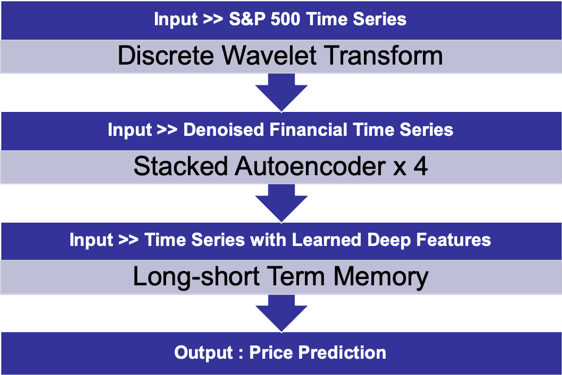
\includegraphics[width=0.6\linewidth]{./figs/flow}%\vspace{-0.4cm}
%\includegraphics[width=0.85\linewidth]{./FIGS/Overview_cropped}%\vspace{-0.2cm}
\caption{Overview of \scheme}
\label{fig-overview}
\end{center}
\vspace{-0.6cm}
\end{figure}

\subsubsection{Denoising using DWT (Wavelet Transform)}
First of all, we apply wavelet transform for data denoising. Wavelet transform has the ability to decompose complex information and patterns into elementary forms. It is applied for data denoising in this project because of its ability to handle non-stationary financial time series data, which is useful in handling highly irregular financial time series. We apply the Haar function as the wavelet basis function because it can not only decompose the financial time series into time and frequency domain but also reduce the processing time significantly. The wavelet transform with the Haar function as a basis has a time complexity of O(n) with n being the size of the time series. We first calculated wavelet coefficients for each data feature column, and designated a threshold to create the signals using thresheld coefficients. 

\subsubsection{Stacked Autoencoder}
After denoising, autoencoders are applied for layer-wise training for the OHLC variables and technical indicators. Single layer AE is a three-layer neural network, the first layer being the input layer and the third layer being the reconstruction layer, respectively. The second layer is the hidden layer, designed to generate the deep feature for this single layer AE. The aim of training the single layer AE is to minimize the error between the input vector and the reconstruction vector. The first step of the forward propagation of single layer AE is mapping the input vector to the hidden layer, while the second step is to reconstruct the input vector by mapping the hidden vector to the reconstruction layer. The activate function can have many alternatives such as sigmoid function, rectified linear unit (ReLU) and hyperbolic tangent. In this project, we set this to be a sigmoid function for all layers. The model learns a hidden feature from input by reconstructing it on the output layer. 

Stacked autoencoders is constructed by stacking a sequence of single-layer AEs layer by layer. The single-layer autoencoder maps the input daily variables into the first hidden vector. After training the first single-layer autoencoder, the hidden layer is reserved as the input layer of the second single-layer autoencoder. Therefore, the input layer of the subsequent AE is the hidden layer of the previous AE. 

For training, Adam optimizer is used for solving the optimization problem in SAEs, and completing parameter optimization. Each layer is trained using the same optimizer as a single-layer AE by and feeds the hidden vector into the subsequent AE. The weights and bias of the reconstruction layer after finishing training each single-layer AE are cast away. Depth plays an important role in SAE because it determines qualities like invariance and abstraction of the extracted feature. In this project, the depth of the SAE will be set to 4 with each layer having 10 hidden units.

\subsubsection{Long-short Term Memory}
After SAEs, we use the time series data as sequence to train the LSTM. LSTM networks consists of an input layer, several hidden layers and an output layer. The number of input layers is the same as the number of features. We choose LSTM because it doesn’t have the problem of vanishing gradients that a Recurrent Neural Network often has. The main drawback of RNN is that it cannot use previously seen data as the size of input sequences becomes larger. LSTM is a gated version of recurrent neural network that solves this problem. 

Another reason we use LSTM is because of the fact that in stock data pattern is the key factor to move the market in technical analysis. Hand-coded models such as clustering or feature extraction are sometimes difficult in time series data such as stock value. Therefore, the main purpose of the LSTM is to capture pattern throughout the time series data. For our LSTM model, the time step size is set to be 4, the batch size to be 60, and the hidden dimension to be 100. For training, we used the mean square error loss with Adam optimizer. 


\subsection{Applying NN with different stock features}
\label{sec-features}
\scheme\ uses different mathematical parameters as features. In stock price it is not enough to see only the price. There are several indicators that is used to predict different signals. \scheme\ uses those signal indicators as different features. However, features are more important for any machine learning model. If the features are good and it is learn-able then the model predictions are more accurate for financial data. Following sections describe the features first, then we describe how \scheme\ uses those in the NN model that we implemented in addition to \scheme\.

\subsubsection{Features}
There are several other feature maps that we use in our experiments are described below.
\begin{itemize}
    \item {\em Moving average convergence divergence (MACD):} MACD gives the convergence divergence of two period running exponential moving average (EMA). We use 12, 26 period EMA for calculating MACD. This features represents how price fluctuates over the period of time.
    
    \item {\em Relative strength index (RSI):} RSI is a momentum indicator that measures the magnitude of recent price changes to evaluate overbought or oversold conditions in the price of a stock or other asset. We choose this features to find out the market momentum at some particular point.
    
    \item {\em Bollinger Band (BB):} A Bollinger Band is a technical analysis tool defined by a set of lines plotted two standard deviations (positively and negatively) away from a simple moving average (SMA) of a stock price. It gives the range for a timeframe to fluctuate. This feature helps to get the highest and lowest point to fluctuate that helps to predict the director of the price.
    
    \item {\em Aroon Indicator:} Aroon is a statistical indicator that is used to identify the trend change in the stock.
    
    \item {\em Pivot points (PP): } PP gives several support and resistance level in price direction. Using this as a features helps to classify the direction of price trend.
    
\end{itemize}

\subsubsection{Model}

\begin{figure}[htpb]
\begin{center}
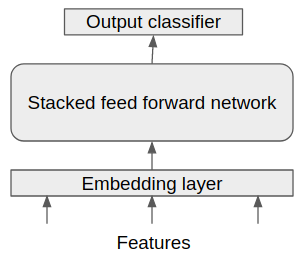
\includegraphics[width=0.35\textwidth]{./figs/stacked_NN}
\vspace{-0.2cm}
\caption{Stacked network with embedding layer for categorical bar prediction}
\label{fig_stackNN}
\end{center}
\vspace{-0.4cm}
\end{figure}


In this experiment we use different features as input and output is different bar predictions. All the bars are divided into several categories according to their body, head and tail (Figure~\ref{fig_stackNN}). At first we make a n-dimension embedding layer with all of our features together. Empirically we see that self learned embedding works better with this model. Embedding layer is passed through n-stacked feed forward network. The model outputs the prediction with softmax layer with cross-entropy loss. Dropout is used to make the training faster.

\subsubsection{A Glance on Implementation  }

Data preparation and handling are entirely conducted in Python 3.7 (Python Software Foundation, 2018), relying on the packages NumPy (Van Der Walt, Colbert, & Varoquaux, 2011), Pandas (McKinney, 2010). The neural network with LSTM are developed with keras (Chollet, 2016) on top of Google TensorFlow, a powerful library for large-scale machine learning on heterogenous systems (Abadi et al., 2015). The AutoEncoder and Wavelet Tranformation are processed by PyWavelets and PyTorch library respectively.

%\section{Lessons Learned}
%\label{sec-lessons}
%During the course of this project, we attempted to extend \scheme\ with several ideas. 
Not all worked out. The failed attempts along with some explanation 
%of the failures 
are as follows: 

%\begin{itemize}
%\begin{enumerate}%[wide, labelwidth=!, labelindent=0pt]    
    %\item 
    {\em 1. Treating $f^{CF}$ and $f^{LCS}$ as regression instead of classification 
    problem:} When we considered $f^{CF}$ and $f^{LCS}$ as regression problems, the neural
    network produced higher prediction error. 
    Therefore, the performance of \scheme\ degraded.

    %\item 
    {\em 2. Neural network to predict the order of genes:} The goal of the fitness 
    score is to provide an order among genes so that the Roulette Wheel algorithm works. So, 
    instead of predicting the actual scores, we tried to predict the order among genes. This 
    idea did not work out because ordering accuracy was worse than that of 
    fitness score based approach.
    
    %\item 
    {\em 3. Multiple predictors:} We experimented with one neural network 
    to predict whether 
    a gene has the fitness score of 0 or not. In case, the fitness score was predicted to be non-zero, we used a different neural network to predict the actual non-zero value. This idea came from the intuition that since many genes have a fitnesss score of 0 (at least for initial generations), we can do a better job predicting those if we use a separate predictor for that purpose. Unfortunately, this ideas also did not work out because the first predictor failed to identify some of good genes that appeared during initial generations.
    
    %\item 
    {\em 4. NS to improve gene quality:} NS can also be used to find better quality genes which can replace the top quality genes that \scheme\ started with (during NS).
    However, since the neural network fitness function is not any more accurate on neighborhood genes than it is on genes generated by the evolutionary algorithm, \scheme\ failed to identify actual better quality genes from the neighborhood in many cases. %That is why, this idea did not benefit \scheme\.     

    %\item 
    {\em 5. Knowing the target program length:} Unsurprisingly, we have found that the \scheme\ finds programs most quickly when we have a priori knowledge of the target program length and maintain all genes at that length.  It is possible to generate the initial genes with some length distribution %centered around some mean 
    and then allow crossover and mutation to change gene length but that increases the time to solution significantly if the target program length is much larger or smaller than the mean initial gene length.  In the future, we plan to explore using a neural network to predict program length to remove the need for a priori knowledge.
    
        %\item {\em }
%\end{itemize}
%\end{enumerate}

\section{Results}
\label{sec-results}
%The goal of this section is to (i) explain the experimental setup, (ii) demonstrate the effectiveness of \scheme\ in synthesizing
%different programs, and (iii) analyze its running time.

%\subsection{Experimental Setup}
%\label{sec-setup}

\subsection{\scheme\ Results}
\label{sec-effectiveness}
As shown in Figure~\ref{fig_loss}, both train and validation losses are improved at some point after 7th sub-data iteration. However, as training reaches the end of our dataset, at around 20th sub-data iterations, we observe spikes of loss increases which may be due to overfitting of the data. To achieve a high accuracy with time series with greater sizes, we will need further hyperparameter tuning to complement this by, for example, adjusting threshold to create signals in our wavelet transformer. 



\begin{figure}[htpb]
\begin{center}
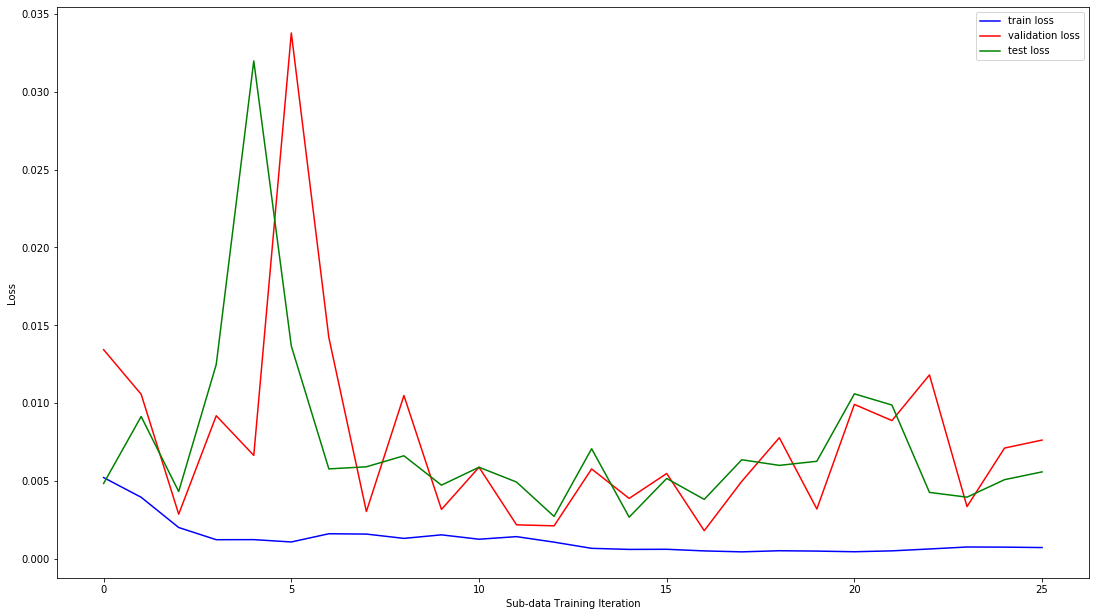
\includegraphics[width=0.9\textwidth]{./figs/lossvsiter}
\vspace{-0.2cm}
\caption{Loss per Sub-dataset Training Iteration}
\label{fig_loss}
\end{center}
\vspace{-0.4cm}
\end{figure}

The actual and predicted price data for S\&P500 are shown in Fig~\ref{fig_loss} and Fig~\ref{fig_actual}. Our model predicts S\&P500 index with reasonable accuracies as shown in Figure~\ref{fig_diff}. At the start, the differences of predicted and actual prices are negligible. However, we observe exponential increase of inaccuracy of over 10 percent of the prices when the stock price plummeted at 2,500 to 3,000th timeframes. The model’s accuracy dropping when the market sentiment is low is further proven by the most recent drop of index prices at around 4,700th timeframe. 

Regarding our model and training schemes, we discovered normalization worsens accuracy compared to when features are scaled manually. We think that this is accountable by that train and test set are normalized at the same time. In other words, there are potential leaks of future information in each time step. Regarding the stacked autoencoder, the intuition was to derive hidden deep features out of the original raw dataset. However, what we think it actually does is to force our data into smaller dimensions with potential loss of important information. We will conduct accuracy comparison with the model without SAE in the future. 

\begin{figure}[htpb]
\begin{center}
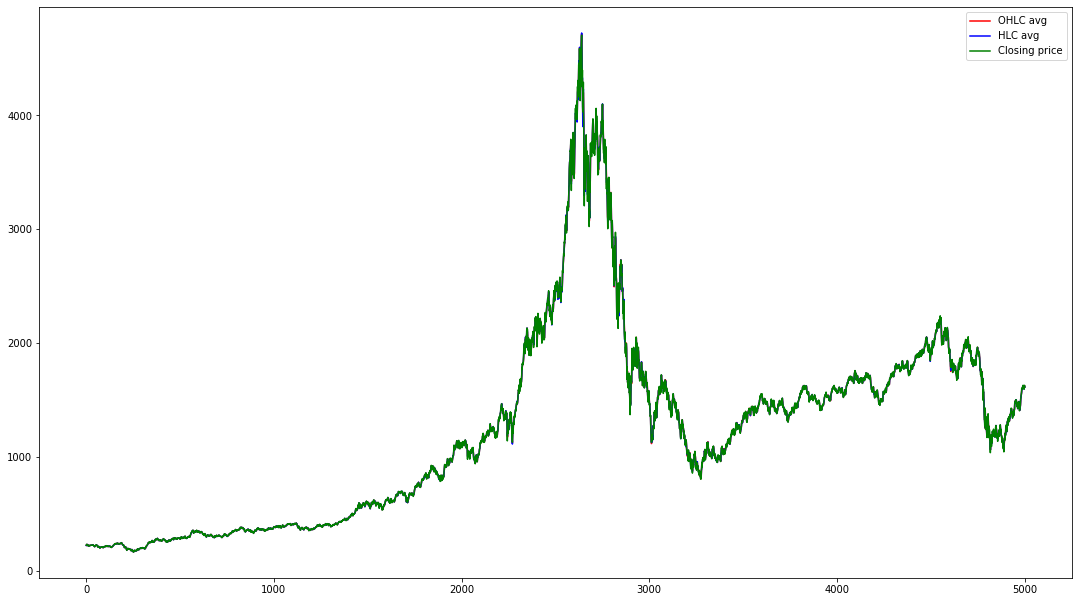
\includegraphics[width=0.9\textwidth]{./figs/actualprice}
\vspace{-0.2cm}
\caption{Actual Data}
%\todo{fix scale from 1 to 41 and 1 to 100}}
\label{fig_actual}
\end{center}
\vspace{-0.6cm}
\end{figure}

\begin{figure}[htpb]
\begin{center}
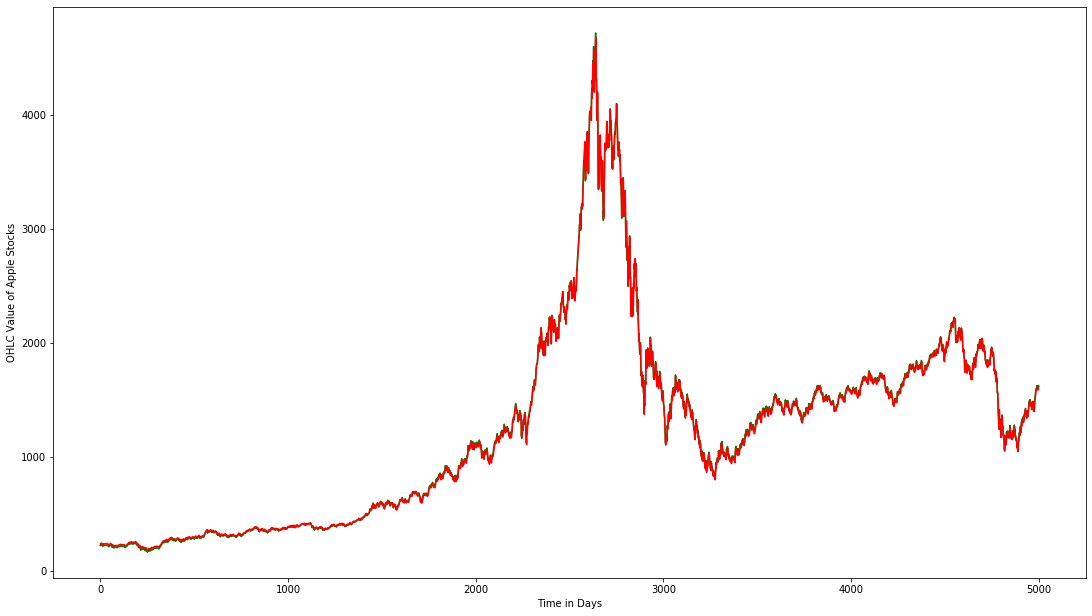
\includegraphics[width=0.9\textwidth]{./figs/predictedprice}
\vspace{-0.2cm}
\caption{Predicted Data}
%\todo{fix scale from 1 to 41 and 1 to 100}}
\label{fig_predict}
\end{center}
\vspace{-0.6cm}
\end{figure}



\begin{figure}[htpb]
\begin{center}
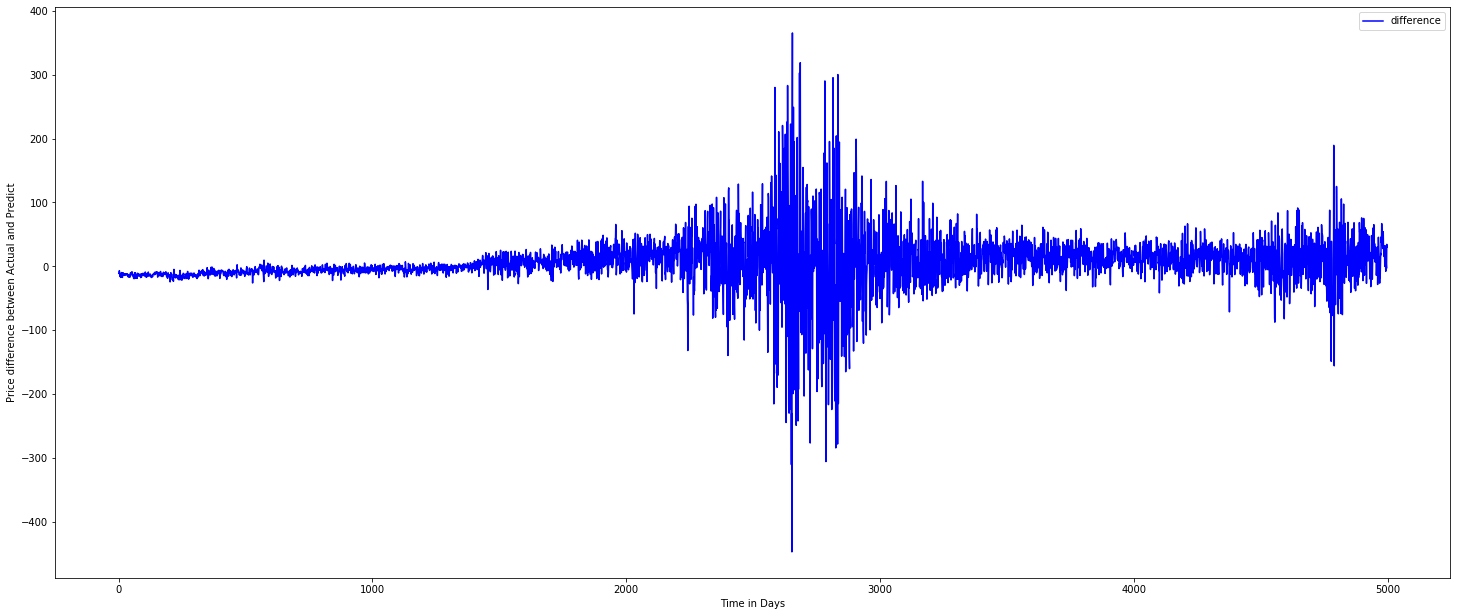
\includegraphics[width=0.9\textwidth]{./figs/pricediff}
\vspace{-0.2cm}
\caption{Difference between Predicted and Actual Prices}
%\todo{fix scale from 1 to 41 and 1 to 100}}
\label{fig_diff}
\end{center}
\vspace{-0.6cm}
\end{figure}



Besides, we tested price history using point-by-point approach and sequence-by-sequence approach in our second architecture. The training and test rate is 0.8. We found that by using 8 epoch, we can achieve the accuracy at 60\%. Though we can find some trends by using the sequence by sequence, the prediction is not stable (Figure 11&12). The point by point prediction figures looks very good but here it is a bit deceptive. We can only predict one data point ahead, based on its all previous history.

\begin{figure}[htpb]
\begin{center}
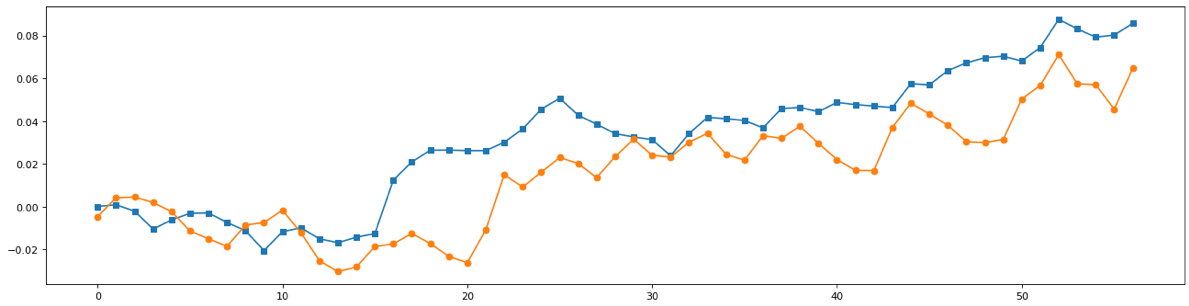
\includegraphics[width=0.9\textwidth]{./figs/PP_2_50.PNG}
\vspace{-0.2cm}
\caption{Point-by-Point prediction (2 Epoch, 50 Batch size)}
%\todo{fix scale from 1 to 41 and 1 to 100}}
\label{fig_predict}
\end{center}
\vspace{-0.6cm}
\end{figure}

\begin{figure}[htpb]
\begin{center}
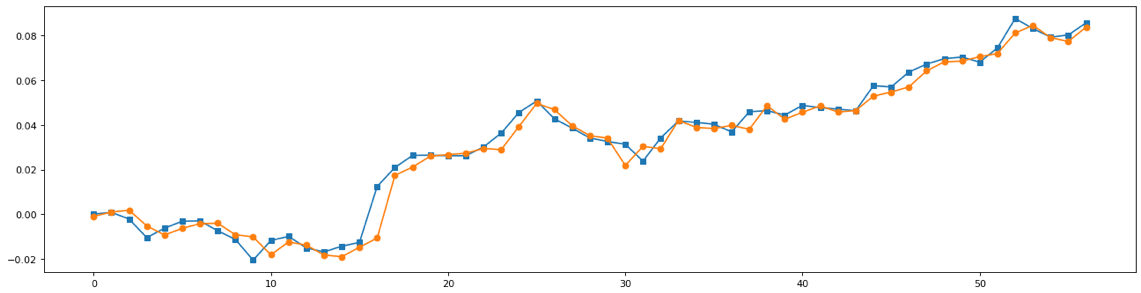
\includegraphics[width=0.9\textwidth]{./figs/PP_8_50.PNG}
\vspace{-0.2cm}
\caption{Point-by-Point prediction (8 Epoch, 50 Batch size)}
%\todo{fix scale from 1 to 41 and 1 to 100}}
\label{fig_predict}
\end{center}
\vspace{-0.6cm}
\end{figure}

\begin{figure}[htpb]
\begin{center}
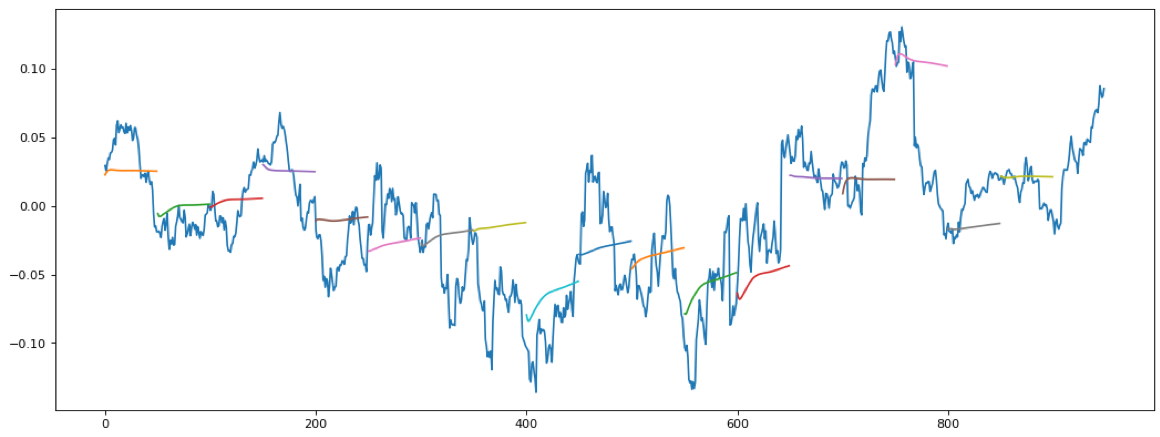
\includegraphics[width=0.9\textwidth]{./figs/SS_2_50.PNG}
\vspace{-0.2cm}
\caption{Sequence-by-Sequence prediction (2 Epoch, 50 Batch size)}
%\todo{fix scale from 1 to 41 and 1 to 100}}
\label{fig_predict}
\end{center}
\vspace{-0.6cm}
\end{figure}

\begin{figure}[htpb]
\begin{center}
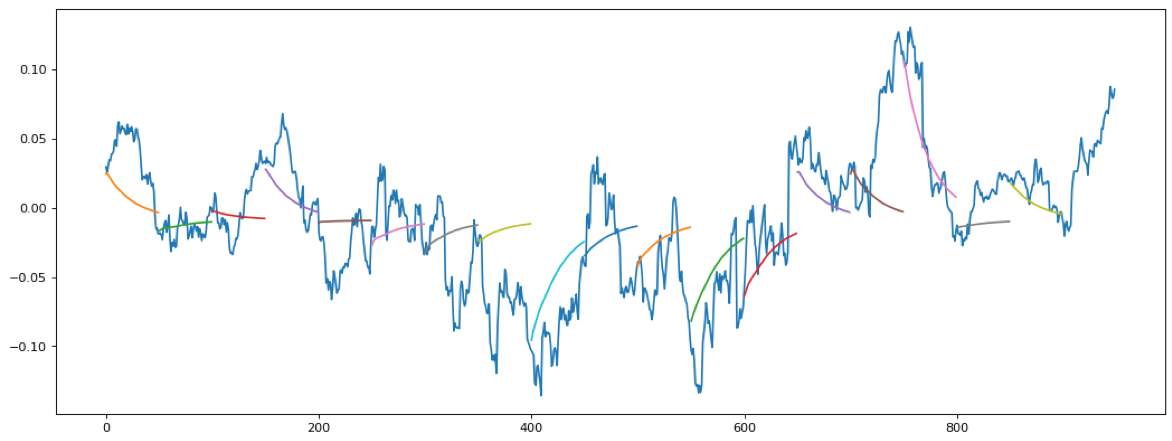
\includegraphics[width=0.9\textwidth]{./figs/SS_4_50.PNG}
\vspace{-0.2cm}
\caption{Sequence-by-Sequence prediction (4 Epoch, 50 Batch size)}
%\todo{fix scale from 1 to 41 and 1 to 100}}
\label{fig_predict}
\end{center}
\vspace{-0.6cm}
\end{figure}


\subsection{Effectiveness of using multiple features in NN model}

\begin{table}[htpb]
  %\scriptsize
  %\parbox{0.3\linewidth}{
  \centering
  \scalebox{0.85}{
  \begin{tabular}{||c| c | c | c ||}
  \hline\hline
  % Recall gives us an idea about when it’s actually yes, how often does it predict yes.
  % Precsion tells us about when it predicts yes, how often is it correct.
   Bar category & Precision & Recall & f1-score \\\hline
   1  & 0.82 & 0.73 & 0.77 \\\hline
   2  & 0.74 & 0.64 & 0.68\\\hline
   3  & 0.62 & 0.67 & 0.64\\\hline
   4  & 0.59 & 0.65 & 0.61\\\hline
   5  & 0.74 & 0.83 & 0.78\\\hline
   6  & 0.89 & 0.82 & 0.85\\\hline
   7  & 0.62 & 0.68 & 0.64\\\hline
   8  & 0.75 & 0.73 & 0.73\\\hline
   9  & 0.82 & 0.83 & 0.82\\\hline
   10 & 0.83 & 0.74 & 0.78\\\hline\hline

  \end{tabular}}
  \vspace{0.3cm}
  \caption{Accuracy of using multiple features in NN model}
  \label{table:features-acc}
  %}
\end{table}

In table \ref{table:features-acc} we describe the precision, recall and f1-score for using the different feature maps to predict different bar category. We divided all the bars into 10 different categories according to their shape. From table \ref{table:features-acc}, bar category 6 has the highest f1-score and category 3 and 7 has the lowest f1-score among all. Overall accuracy of our model is 67\%.


\section{Related Work}
\label{sec-rel}
% !TEX root =  main.tex

Initial evidence has been established that machine learning techniques are capable of identifying (non- linear) structures in financial market data, see Huck (2009, 2010),  
Takeuchi and Lee (2013) , Moritz and Zimmermann (2014) , Dixon, Klabjan, and Bang (2015) , and further references in Atsalakis and Valavanis (2009) as well as Sermpinis, Theofilatos, Karathana- sopoulos, Georgopoulos, and Dunis (2013). The relevant work on deep learning applied to finance has introduced the convolutional neural networks, deep belief networks. For example, Ding et al.~\cite{ding2015deep} combine the neural tensor network and the deep convolutional neural network to predict the short-term and long-term influences of events on stock price movements. Other than that, certain works use deep belief networks in financial market prediction, for example, Yoshihara et al. ~\cite{yoshihara2014predicting}, Shen et al. ~\cite{shen2015forecasting} and Kuremoto et al. ~\cite{kuremoto2014time}.
 

\section{Future work}
\label{sec-future}
% !TEX root =  main.tex

There are several path to look into in extending our work. Among them we thought of doing the following as our future work. 

1. We want to show different deep neural network model comparison on stock analysis and find out the best fitted model for our case. 

2. Different benchmark comparison with market alpha. 

3. Make a framework that is easily extendable with different prediction model. 

%\section{Background}
%\label{sec-back}
%\input{back}


%\section{\scheme: Root Cause Analysis}
%\label{sec-desc}
%% overview
% Encoding
% Crossover \& Mutation
% Fitness function:
% - CF
% - LCS
% - Deepcoder
% Neighborhood search:
% - parametric neighborhood search
% - BFS
% - DFS
% In implementation/result section, talk about training data generation

%We will start with a high level overview of \scheme\ %followed by the detailed description of each component.

%\subsection{Overview}
%Figure~\ref{fig-overview} shows the high level system diagram of \scheme. 

In the following sections we describe two approaches with different model architecture and features. \\ 
{\em First}, we describe the \scheme\ model that tries to analyse prices with discrete wavelet transform with LSTM. \\
{\em Second}, in addition to this, we describe stacked NN trained with multiple features with embedding layer for performance comparison.

\subsection{ Model}
\subsubsection{Overview}
\label{sec-jee}

As mention, our dataset uses 10 years’ daily price data of S\&P500 index. Each row of daily stock price information includes OHLC (Open, High, Low, Close), technical indicators (MACD, CCI, ATR, BOLL, EMA20, MA10, MTM6, MA5, MTM12, ROC, SMI, WVAD), and macroeconomic variables (US Dollar Index, Federal Fund Rate). Instead of normalization, we applied manual scaling of these input features so that they can have similar orders of magnitude. For each 'sub-dataset training iteration', we divided the dataset into sub-datasets with each having 600 days of data, which is a bit more than 2 years of data. Our step size was set to 2 months as we thought it was a reasonable timeframe where each price data during that time can affect the opening price of that stock after 2 months. Specifically, for each sub-data, we used the most recent 60 days of data as the test data, the second most recent 60 days as the validation, and the rest as the training data. 

As we initially planned, we implemented a model (Figure~\ref{fig-overview}) that takes denoised inputs that are preprocessed via wavelet transform, and trains based on a 4-layer stacked autoencoder and subsequent Long-short term memory neural network.

\begin{figure}[htpb]
\begin{center}
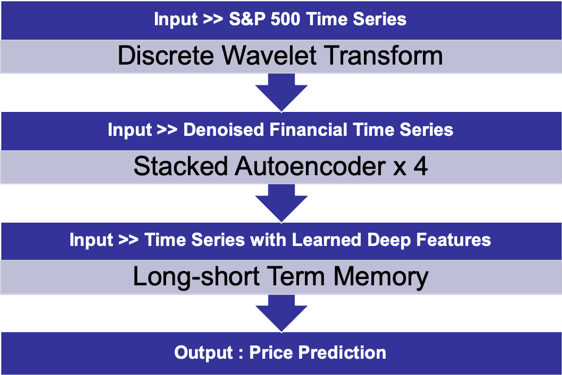
\includegraphics[width=0.6\linewidth]{./figs/flow}%\vspace{-0.4cm}
%\includegraphics[width=0.85\linewidth]{./FIGS/Overview_cropped}%\vspace{-0.2cm}
\caption{Overview of \scheme}
\label{fig-overview}
\end{center}
\vspace{-0.6cm}
\end{figure}

\subsubsection{Denoising using DWT (Wavelet Transform)}
First of all, we apply wavelet transform for data denoising. Wavelet transform has the ability to decompose complex information and patterns into elementary forms. It is applied for data denoising in this project because of its ability to handle non-stationary financial time series data, which is useful in handling highly irregular financial time series. We apply the Haar function as the wavelet basis function because it can not only decompose the financial time series into time and frequency domain but also reduce the processing time significantly. The wavelet transform with the Haar function as a basis has a time complexity of O(n) with n being the size of the time series. We first calculated wavelet coefficients for each data feature column, and designated a threshold to create the signals using thresheld coefficients. 

\subsubsection{Stacked Autoencoder}
After denoising, autoencoders are applied for layer-wise training for the OHLC variables and technical indicators. Single layer AE is a three-layer neural network, the first layer being the input layer and the third layer being the reconstruction layer, respectively. The second layer is the hidden layer, designed to generate the deep feature for this single layer AE. The aim of training the single layer AE is to minimize the error between the input vector and the reconstruction vector. The first step of the forward propagation of single layer AE is mapping the input vector to the hidden layer, while the second step is to reconstruct the input vector by mapping the hidden vector to the reconstruction layer. The activate function can have many alternatives such as sigmoid function, rectified linear unit (ReLU) and hyperbolic tangent. In this project, we set this to be a sigmoid function for all layers. The model learns a hidden feature from input by reconstructing it on the output layer. 

Stacked autoencoders is constructed by stacking a sequence of single-layer AEs layer by layer. The single-layer autoencoder maps the input daily variables into the first hidden vector. After training the first single-layer autoencoder, the hidden layer is reserved as the input layer of the second single-layer autoencoder. Therefore, the input layer of the subsequent AE is the hidden layer of the previous AE. 

For training, Adam optimizer is used for solving the optimization problem in SAEs, and completing parameter optimization. Each layer is trained using the same optimizer as a single-layer AE by and feeds the hidden vector into the subsequent AE. The weights and bias of the reconstruction layer after finishing training each single-layer AE are cast away. Depth plays an important role in SAE because it determines qualities like invariance and abstraction of the extracted feature. In this project, the depth of the SAE will be set to 4 with each layer having 10 hidden units.

\subsubsection{Long-short Term Memory}
After SAEs, we use the time series data as sequence to train the LSTM. LSTM networks consists of an input layer, several hidden layers and an output layer. The number of input layers is the same as the number of features. We choose LSTM because it doesn’t have the problem of vanishing gradients that a Recurrent Neural Network often has. The main drawback of RNN is that it cannot use previously seen data as the size of input sequences becomes larger. LSTM is a gated version of recurrent neural network that solves this problem. 

Another reason we use LSTM is because of the fact that in stock data pattern is the key factor to move the market in technical analysis. Hand-coded models such as clustering or feature extraction are sometimes difficult in time series data such as stock value. Therefore, the main purpose of the LSTM is to capture pattern throughout the time series data. For our LSTM model, the time step size is set to be 4, the batch size to be 60, and the hidden dimension to be 100. For training, we used the mean square error loss with Adam optimizer. 


\subsection{Applying NN with different stock features}
\label{sec-features}
\scheme\ uses different mathematical parameters as features. In stock price it is not enough to see only the price. There are several indicators that is used to predict different signals. \scheme\ uses those signal indicators as different features. However, features are more important for any machine learning model. If the features are good and it is learn-able then the model predictions are more accurate for financial data. Following sections describe the features first, then we describe how \scheme\ uses those in the NN model that we implemented in addition to \scheme\.

\subsubsection{Features}
There are several other feature maps that we use in our experiments are described below.
\begin{itemize}
    \item {\em Moving average convergence divergence (MACD):} MACD gives the convergence divergence of two period running exponential moving average (EMA). We use 12, 26 period EMA for calculating MACD. This features represents how price fluctuates over the period of time.
    
    \item {\em Relative strength index (RSI):} RSI is a momentum indicator that measures the magnitude of recent price changes to evaluate overbought or oversold conditions in the price of a stock or other asset. We choose this features to find out the market momentum at some particular point.
    
    \item {\em Bollinger Band (BB):} A Bollinger Band is a technical analysis tool defined by a set of lines plotted two standard deviations (positively and negatively) away from a simple moving average (SMA) of a stock price. It gives the range for a timeframe to fluctuate. This feature helps to get the highest and lowest point to fluctuate that helps to predict the director of the price.
    
    \item {\em Aroon Indicator:} Aroon is a statistical indicator that is used to identify the trend change in the stock.
    
    \item {\em Pivot points (PP): } PP gives several support and resistance level in price direction. Using this as a features helps to classify the direction of price trend.
    
\end{itemize}

\subsubsection{Model}

\begin{figure}[htpb]
\begin{center}
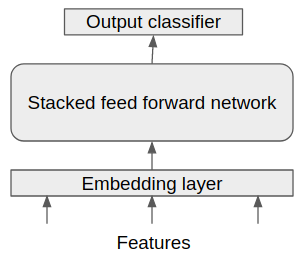
\includegraphics[width=0.35\textwidth]{./figs/stacked_NN}
\vspace{-0.2cm}
\caption{Stacked network with embedding layer for categorical bar prediction}
\label{fig_stackNN}
\end{center}
\vspace{-0.4cm}
\end{figure}


In this experiment we use different features as input and output is different bar predictions. All the bars are divided into several categories according to their body, head and tail (Figure~\ref{fig_stackNN}). At first we make a n-dimension embedding layer with all of our features together. Empirically we see that self learned embedding works better with this model. Embedding layer is passed through n-stacked feed forward network. The model outputs the prediction with softmax layer with cross-entropy loss. Dropout is used to make the training faster.

\subsubsection{A Glance on Implementation  }

Data preparation and handling are entirely conducted in Python 3.7 (Python Software Foundation, 2018), relying on the packages NumPy (Van Der Walt, Colbert, & Varoquaux, 2011), Pandas (McKinney, 2010). The neural network with LSTM are developed with keras (Chollet, 2016) on top of Google TensorFlow, a powerful library for large-scale machine learning on heterogenous systems (Abadi et al., 2015). The AutoEncoder and Wavelet Tranformation are processed by PyWavelets and PyTorch library respectively.


%\section{Implementation}
%\label{sec-impl}
%\input{impl}


%\section{Additional Issues}
%\label{sec-additional}
%\input{additional}


%\section{Experimental Results}
%\label{sec-results}
%\input{results_new}

%\section{Limitations and Future Work}
%\label{sec-limit}
%\input{limit}

%\section{Related Work}
%\label{sec-rel}
%% !TEX root =  main.tex

Initial evidence has been established that machine learning techniques are capable of identifying (non- linear) structures in financial market data, see Huck (2009, 2010),  
Takeuchi and Lee (2013) , Moritz and Zimmermann (2014) , Dixon, Klabjan, and Bang (2015) , and further references in Atsalakis and Valavanis (2009) as well as Sermpinis, Theofilatos, Karathana- sopoulos, Georgopoulos, and Dunis (2013). The relevant work on deep learning applied to finance has introduced the convolutional neural networks, deep belief networks. For example, Ding et al.~\cite{ding2015deep} combine the neural tensor network and the deep convolutional neural network to predict the short-term and long-term influences of events on stock price movements. Other than that, certain works use deep belief networks in financial market prediction, for example, Yoshihara et al. ~\cite{yoshihara2014predicting}, Shen et al. ~\cite{shen2015forecasting} and Kuremoto et al. ~\cite{kuremoto2014time}.
 


\section{Conclusion}
\label{sec-conc}
% !TEX root =  main.tex

In this paper, we presented an stock prediction framework called \scheme\ which consists of various types of NNs. We attempted to predict the stock value with different network topologies with different features vector. Here we show how NN can be used as a good stock predictor that can easily trained compared to other machine learning model. We proposed different neural network architecture and
contrasted them against different hand-based state-of-the art statistical indicator and machine learning technique. We shown that given enough data and different features vector neural network performs can better than other machine learning model and it also becomes much easier to train.




%\input{variance_term}

%\bibliographystyle{plain}
\bibliographystyle{abbrv}
%\bibliographystyle{abbrvnat}
%\bibliographystyle{ACM-Reference-Format}
\bibliography{main}

%\newpage
%\appendix
%\section{Appendix A: Our List DSL}
%\label{sec-appendix-dsl}
%In this appendix, we provide more details about the list DSL that \scheme\ uses to generate programs.  Our list DSL has only two implicit data types, integer and list of integer.  A program in this DSL is a sequence of statements, each of which is a call to one of the 41 functions defined in the DSL.  There are no explicit variables, nor conditionals, nor explicit control flow operations in the DSL, although many of the functions in the DSL are high-level and contain implicit conditionals and control flow within them.  Each of the 41 functions in the DSL takes one or two arguments, each being of integer or list of integer type, and returns exactly one output, also of integer or list of integer type.  Given these rules, there are 10 possible function signatures.  However, only 5 of these signatures occur for the functions we chose to be part of the DSL.  The following sections are broken down by the function signature, wherein all the functions in the DSL having that signature are described.

Instead of named variables, each time a function call requires an argument of a particular type, our DSL's runtime searches backwards and finds the most recently executed function that returns an output of the required type and then uses that output as the current function's input.  Thus, for the first statement in the program, there will be no previous function's output from which to draw the arguments for the first function.  When there is no previous output of the correct type, then our DSL's runtime looks at the arguments to the program itself to provide those values.  Moreover, it is possible for the program's inputs to not provide a value of the requested type.  In such cases, the runtime provides a default value for missing inputs, 0 in the case of integer and an empty list in the case of list of integer.  For example, let us say that a program is given a list of integer as input and that the first three functions called in the program each consume and produce a list of integer.  Now, let us assume that the fourth function called takes an integer and a list of integer as input.  The list of integer input will use the list of integer output from the previous function call.  The DSL runtime will search backwards and find that none of the previous function calls produced integer output and that no integer input is present in the program's inputs either.  Thus, the runtime would provide the value 0 as the integer input to this fourth function call.  The final output of a program is the output of the last function called.

Thus, our language is defined in such a way that so long as the program consists only of calls to one of the 41 functions provided by the DSL, that these programs are valid by construction. 
Each of the 41 functions is guaranteed to finish in a finite time and there are no looping constructs in the DSL and thus programs in our DSL are guaranteed to finish.  This property allows our system to not have to monitor the programs that they execute to detect potentially infinite loops.  Moreover, so long as the implementations of those 41 functions are secure and have no potential for memory corruption then programs in our DSL are similarly guaranteed to be secure and not crash and thus we do not require any sand-boxing techniques.  When our system performs crossover between two candidate programs, any arbitrary cut points in both of the parent programs will result in a child program that is also valid by construction.  Thus, our system need not test that programs created via crossover or mutation are valid.

In the following sections, \emph{[]} is used to indicate the type list of integer whereas \emph{int} is used to indicate the integer type.  The type after the arrow is used to indicate the output type of the function.

\subsection{Functions with the signature $\emph{[]} \rightarrow \emph{int}$}
There are 9 functions in our DSL that take a list of integer as input and return an integer as output.
\subsubsection{HEAD (Function 6)}
This function returns the first item in the input list.  If the list is empty, a 0 is returned.
\subsubsection{LAST (Function 7)}
This function returns the last item in the input list.  If the list is empty, a 0 is returned.
\subsubsection{MINIMUM (Function 8)}
This function returns the smallest integer in the input list.  If the list is empty, a 0 is returned.
\subsubsection{MAXIMUM (Function 9)}
This function returns the largest integer in the input list.  If the list is empty, a 0 is returned.
\subsubsection{SUM (Function 11)}
This functions returns the sum of all the integers in the input list.  If the list is empty, a 0 is returned.
\subsubsection{COUNT (Function 2-5)}
This function returns the number of items in the list that satisfy the criteria specified by the additional lambda.  Each possible lambda is counted as a different function.  Thus, there are 4 COUNT functions having lambdas: >0, <0, odd, even.

\subsection{Functions with the signature $\emph{[]} \rightarrow \emph{[]}$}
There are 21 functions in our DSL that take a list of integer as input and produce a list of integer as output.
\subsubsection{REVERSE (Function 29)}
This function returns a list containing all the elements of the input list but in reverse order.
\subsubsection{SORT (Function 35)}
This function returns a list containing all the elements of the input list in sorted order.
\subsubsection{MAP (Function 19-28)}
This function applies a lambda to each element of the input list and creates the output list from the outputs of those lambdas.  Let $I_n$ be the nth element of the input list to MAP and let $O_n$ be the nth element of the output list from Map.  MAP produces an output list such that $O_n$=lambda($I_n$) for all n.  There are 10 MAP functions corresponding to the following lambdas: +1,-1,*2,*3,*4,/2,/3,/4,*(-1),\^{}2.
\subsubsection{FILTER (Function 14-17)}
This function returns a list containing only those elements in the input list satisfying the criteria specified by the additional lambda.  Ordering is maintained in the output list relative to the input list for those elements satisfying the criteria.  There are 4 FILTER functions having the lambdas: >0, <0, odd, even.
\subsubsection{SCANL1 (Function 30-34)}
Let $I_n$ be the nth element of the input list to SCANL1 and let $O_n$ be the nth element of the output list from SCANL1.  This function produces an output list as follows:

\[ \begin{cases} 
      $O\_n$=$I\_n$ & $n$==$0$ \\
      $O\_n$=lambda($I\_n$,$O\_{n-1}$) & $n$>$0$ 
   \end{cases}
\]

There are 5 SCANL1 functions corresponding to the following lambdas: +, -, *, min, max.

\subsection{Functions with the signature $\emph{int,{[]}} \rightarrow \emph{[]}$}
There are 4 functions in our DSL that take an integer and a list of integer as input and produce a list of integer as output.
\subsubsection{TAKE (Function 36)}
This function returns a list consisting of the first N items of the input list where N is the smaller of the integer argument to this function and the size of the input list.
\subsubsection{DROP (Function 13)}
This function returns a list in which the first N items of the input list are omitted, where N is the integer argument to this function.
\subsubsection{DELETE (Function 12)}
This function returns a list in which all the elements of the input list having value X are omitted where X is the integer argument to this function.
\subsubsection{INSERT (Function 18)}
This function returns a list where the value X is appended to the end of the input list, where X is the integer argument to this function.

\subsection{Functions with the signature $\emph{[],[]} \rightarrow \emph{[]}$}
There is only one function in our DSL that takes two lists of integers and returns another list of integers.
\subsubsection{ZIPWITH (Function 37-41)}
This function returns a list whose length is equal to the length of the smaller input list.  Let $O_n$ be the nth element of the output list from ZIPWITH.  Moreover, let $I^1_n$ and $I^2_n$ be the nth elements of the first and second input lists respectively.  This function creates the output list such that $O_n$=lambda($I^1_n$, $I^2_n$).  There are 5 ZIPWITH functions corresponding to the following lambdas: +, -, *, min, max.

\subsection{Functions with the signature $\emph{int,[]} \rightarrow \emph{int}$}
There are two functions in our DSL that take an integer and list of integer and return an integer.
\subsubsection{ACCESS (Function 1)}
This function returns the Nth element of the input list, where N is the integer argument to this function.  If N is less than 0 or greater than the length of the input list then 0 is returned.
\subsubsection{SEARCH (Function 10)}
This function return the position in the input list where the value X is first found, where X is the integer argument to this function.  If no such value is present in the list, then -1 is returned.

%\section{Appendix B: System}
%\label{sec-appendix-system}
%\subsection{Hyper parameters for evolutionary algorithm and neural network}
\begin{itemize}
\item{Evolutionary Algorithm:}
    \begin{itemize}
        \item{} Gene pool size: 100
        \item{} Number of reserve gene in each generation: 20
        \item{} Maximum number of generation: 30,000
        \item{} Gene length: 4
        \item{} Crossover rate: 40\%
        \item{} Mutation rate: 30\%
    \end{itemize}
\item{Neural Network Training:}
    \begin{itemize}
        \item{} Loss: Categorical Cross-Entropy
        \item{} Optimizer: Adam
        \item{} 3 hidden layers with neurons 48, 24, 12
        \item{} Activation function: Sigmoid in hidden layers and Softmax in output layer.
    \end{itemize}

\end{itemize}

\subsection{How we generate training dataset for the neural network}
 
For our two approaches ($f^{LCS}$ and $f^{FP}$), we created 3 types of data sets for 3 different models ($IO$, $IO^2$, $IO^\delta$). We used 50,000 programs as base program and to compare we chose 150 different other programs. These two sets of programs are compared with each other to get the number of common function or longest common sub-sequence between them. In each comparison we created 100 input-output examples that lead to total 750 million data points. For $IO$ model we generated our dataset from the base program but for $IO^2$ and $IO^\delta$ model we need another output that we created with the comparable program by passing the inputs. Each input or output were padded to fixed 12 dimension and  were joined together. For the $IO^\delta$ model we took absolute difference between input and corresponding two different outputs. Also add the information of dimension difference of two output. Thus for the three models input dimension were 24 ($IO$), 36 ($IO^2$), 25 ($IO^\delta$).

With our training programs and given input-output examples we created our dataset. We split out the dataset into training and testing set in a ratio of 3:1. We also randomized the dataset before splitting. Data were normalized before feeding into the neural network. 


\subsection{Training of Neural Network}

We used 3 hidden layers in our model. Our models predicted common functions/longest common subsequence between the target programs and generated programs from EA by using input-output examples. We predicted that value as a classification output.

For the Deepcoder model, we used 3 hidden layers with 256 neurons each. We passed the input through the embedding layer connected to the input neurons. We took average for the input-output examples and predicted function probability.

\end{document}
